\documentclass[conference]{IEEEtran}
\IEEEoverridecommandlockouts
% The preceding line is only needed to identify funding in the first footnote. If that is unneeded, please comment it out.
\usepackage{cite}
\usepackage{amsmath,amssymb,amsfonts}
\usepackage{algorithmic}
\usepackage{graphicx}
\usepackage{textcomp}
\usepackage{xcolor}
\usepackage[ngerman]{babel}
\usepackage[acronym]{glossaries}
%\usepackage{setspace}
\makeglossaries
\newacronym{sg}{SG}{Serious Games}
\newacronym{xr}{XR}{Extended Reality}
\newacronym{vr}{VR}{Virtual Reality}
\newacronym{ar}{AR}{Augmented Reality}
\newacronym{cg}{CG}{Computer Grafik}
\newacronym{gbl}{GBL}{Game-Based Learning}


\def\BibTeX{{\rm B\kern-.05em{\sc i\kern-.025em b}\kern-.08em
    T\kern-.1667em\lower.7ex\hbox{E}\kern-.125emX}}
\begin{document}

\title{Anwendung des Serious Gamings mittels erweiterter Realität in der hochschuldidaktischen Lehre\\
%{\footnotesize \textsuperscript{*}Wissenschaftliches Arbeiten WS2021/2022 Fachhochschule Aachen}
%\thanks{Identify applicable funding agency here. If none, delete this.}
}


\author{\IEEEauthorblockN{1\textsuperscript{st} Marcel Werner Heinrich Friedrich Ochsendorf}
\IEEEauthorblockA{\textit{Fachhochschule Aachen} \\
\textit{Fachbereich 5 Elektrotechnik und Informationstechnik}\\
Aachen, Deutschland \\
marcel.ochsendorf@alumni.fh-aachen.de}
%\and
}

\maketitle

%-----------------------------------------------------------------------------------------------------------------------------------------------
% \gls{uscf}
\begin{abstract}
Die Integration moderner Medien in die hochschuldidaktische Lehre hat seit der Jahrtausendwende stetig an Bedeutung gewonnen.
Dieses Papier zeigt eine Möglichkeit zur Vermittlung von Wissen und die Motivation zum Lernen mittels \gls{xr} am Beispiel der Vorlesung
\gls{cg} basierend auf den Erkenntnissen von bereits etablierten Lösungen.
Wissen soll hierbei durch softwarebasierte Spiele, den \gls{sg}, vermittelt werden.
Anders als bei existierenden 2D Display-Anwendungen werden bei \gls{xr} visuelle Informationen mittels virtuellen Umgebungen, Objekten und Interaktionen mit diesen vermittelt.
Die Studierenden können Situationen aus einem Blickwinkel ihrer Wahl erkunden und erlernen und können zudem durch Wiederholen von Aufgaben in verschiedenen Blickwinkeln
ihr Wissen anpassen.
Meist ohne unterstützende Lehrkörper werden Studierende innerhalb dieser Umgebung einzeln oder in Gruppen mit Aufgaben und Informationen konfrontiert,
welche die Interaktions- und Imaginationsinstinkte ansprechen.
Insbesondere die untersuchte Lehrveranstaltung \gls{cg} ermöglicht viele Umsetzungen des \gls{sg}-Ansatzes, da technologische Themenbereiche und die grafischen Unterschiede
mittels \gls{xr} hervorgehoben werden können.
\end{abstract}

\begin{IEEEkeywords}
Serious Gaming (\gls{sg}), \gls{vr}, Extended Reality (\gls{xr}), Computer Grafik (\gls{cg})
\end{IEEEkeywords}

\section{Einleitung}
Die Anwendung von 3D-Technologien und virtuellen Umgebungen hat in der Vergangenheit stark zugenommen
und wird erheblich weiter steigen, wie Statistiken aus den USA zeigen\cite{eduxrvrar2020usa}.
Die Variationen und Möglichkeiten der \gls{vr}-Technologien werden durch das rapide Wachstum von schneller und erschwingliche Hardware, Software und Netzwerken begünstigt\cite{evallearningmixedreality2020}.
Mit Veränderungen des alltäglichen Umfelds und dem wachsenden Umfang von Wissen muss sich auch die Lehre diesen Veränderungen anpassen und kann daraus auch
Nutzen ziehen.
\gls{gbl} nutzt jene Technologien, um Lehrinhalte und Informationen spielerisch an Nutzer, in diesem Falle Studierende, zu vermitteln und somit die
Motivation zum Lernen zu steigern.
Die Möglichkeiten der Umsetzung sind vielfältig und bieten verschiedene Vor- und Nachteile.
Die Umsetzung ist komplex, da anders als bei 2D-Display-Anwendungen die \gls{xr}-Technologien zusammen mit Interaktionsoptionen für jeden Studierenden
die finanzielle Belastung selten aufgebracht werden kann. Für ein einzelnes Fach ist der Aufwand groß. Zudem ist die Umsetzung insbesondere für mehrere Studierende zeitintensiver.
Die Ergebnisse für die Lehre sind fast ausschließlich positiv und werden in der Evaluation dieses Papiers gesondert beleuchtet.
Studierende reflektieren erlerntes Wissen besser und nehmen den Lehrprozess positiver wahr;
mehr als Zweidrittel der Studierenden befürworten eine verstärkte Integration von \gls{xr} in der Lehre\cite{a7}.\\


Im Folgenden werden die verschiedenen Begriffe definiert und voneinander abgegrenzt;
anschließend werden Möglichkeiten des Einsatzes von \gls{xr} in der Lehre der \gls{cg} der Fachhochschule Aachen vorgestellt.

%-----------------------------------------------------------------------------------------------------------------------------------------------
%ERLÄUTERUNGEN

\section{Serious Gaming und extended Reality Technologien}

Um \gls{sg} in der Lehre der \gls{cg} evaluieren und einsetzen zu können, werden zuerst die Themenbereiche voneinander abgegrenzt und erläutert.

\subsection{Game-Based Learning (\gls{gbl})}
Mittels \gls{gbl} soll spielerisch Wissen vermittelt werden. Man unterscheidet in Board Game Simulations und Digital \gls{gbl}.
Erstere sind rein haptische und nicht digitale Spiele, wie beispielsweise Schach, welches strategisches Denken lehrt und fördert.
Letztere beinhalten die Wissensvermittlung mittels digitaler Möglichkeiten und ermöglichen genau wie Ersteres regelbasiert Aktionen und Interaktionen,
durch den digitalen Anteil ist die Varianz deutlich erhöht und die Komplexität wird gesteigert.
Zudem können zusätzliche Komponenten, wie Ton, Bild oder Reaktionen verwendet und die Aufmerksamkeit des Anwenders gesteuert werden.
Der Lernprozess soll durch das Spielen nicht nur kognitiv, sondern durch eine Vielzahl an Sinnesorganen angesprochen werden, sodass die Erinnerungsleistung der
synaptischen Repräsentation im Gehirn erhöht wird\cite{fabulagames}.
Mittels digitaler Medien kann zudem das Spiel dezentral und / oder vernetzt umgesetzt werden\cite{a3}.

\begin{figure}[htbp]
\centerline{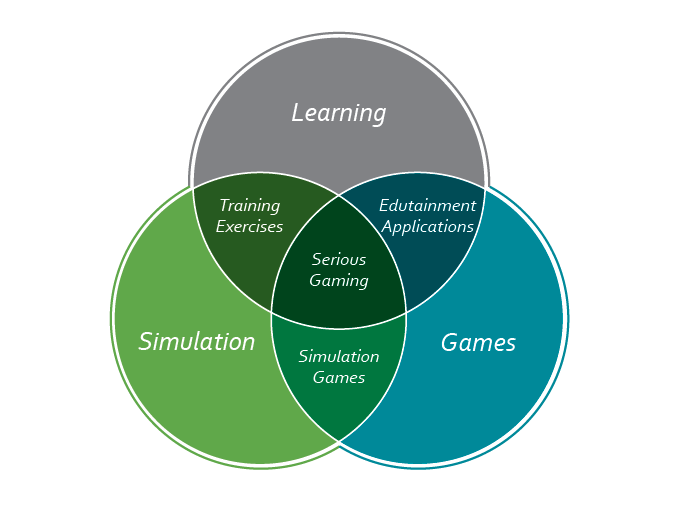
\includegraphics[width=8cm]{serious-games.png}}
\caption{Definition Serious Games.\cite{a10}}
\label{sgdef_fig}
\end{figure}


\subsection{Serious Gaming (\gls{sg})}
Mit dem Ziel der Vermittlung von Inhalten und Kompetenzen sind \gls{sg}s, Instrumente zur Wissensvermittlung (s. Abbildung \ref{sgdef_fig}).
Wörtlich übersetzt bedeutet es ``Spiel mit ernsthaftem (Lern-)Ziel''.
Unterhaltung ist nur ein untergeordnetes Ziel dieser Spiele, jedoch nicht unbedeutend, da der Anwender im Spiel motiviert werden soll.
Einerseits kann erlerntes Wissen vertieft und wiederholt und andererseits neues Wissen erlernt werden.
Es ist zu beachten, dass \gls{sg} auch 2D und / oder nicht \gls{xr}-basierende Spiele beinhaltet.
Demnach können auch nicht digitale Spiele, wie Board Game Simulations, den \gls{sg} zugeordnet werden.
Nachfolgend wird den \gls{sg}s nur in Bezug auf \gls{xr}-basierte Spiele betrachtet.
Nicht digitale oder Spiele für 2D Ausgabegeräte werden hierbei nicht berücksichtigt.

\begin{figure}[htbp]
\centerline{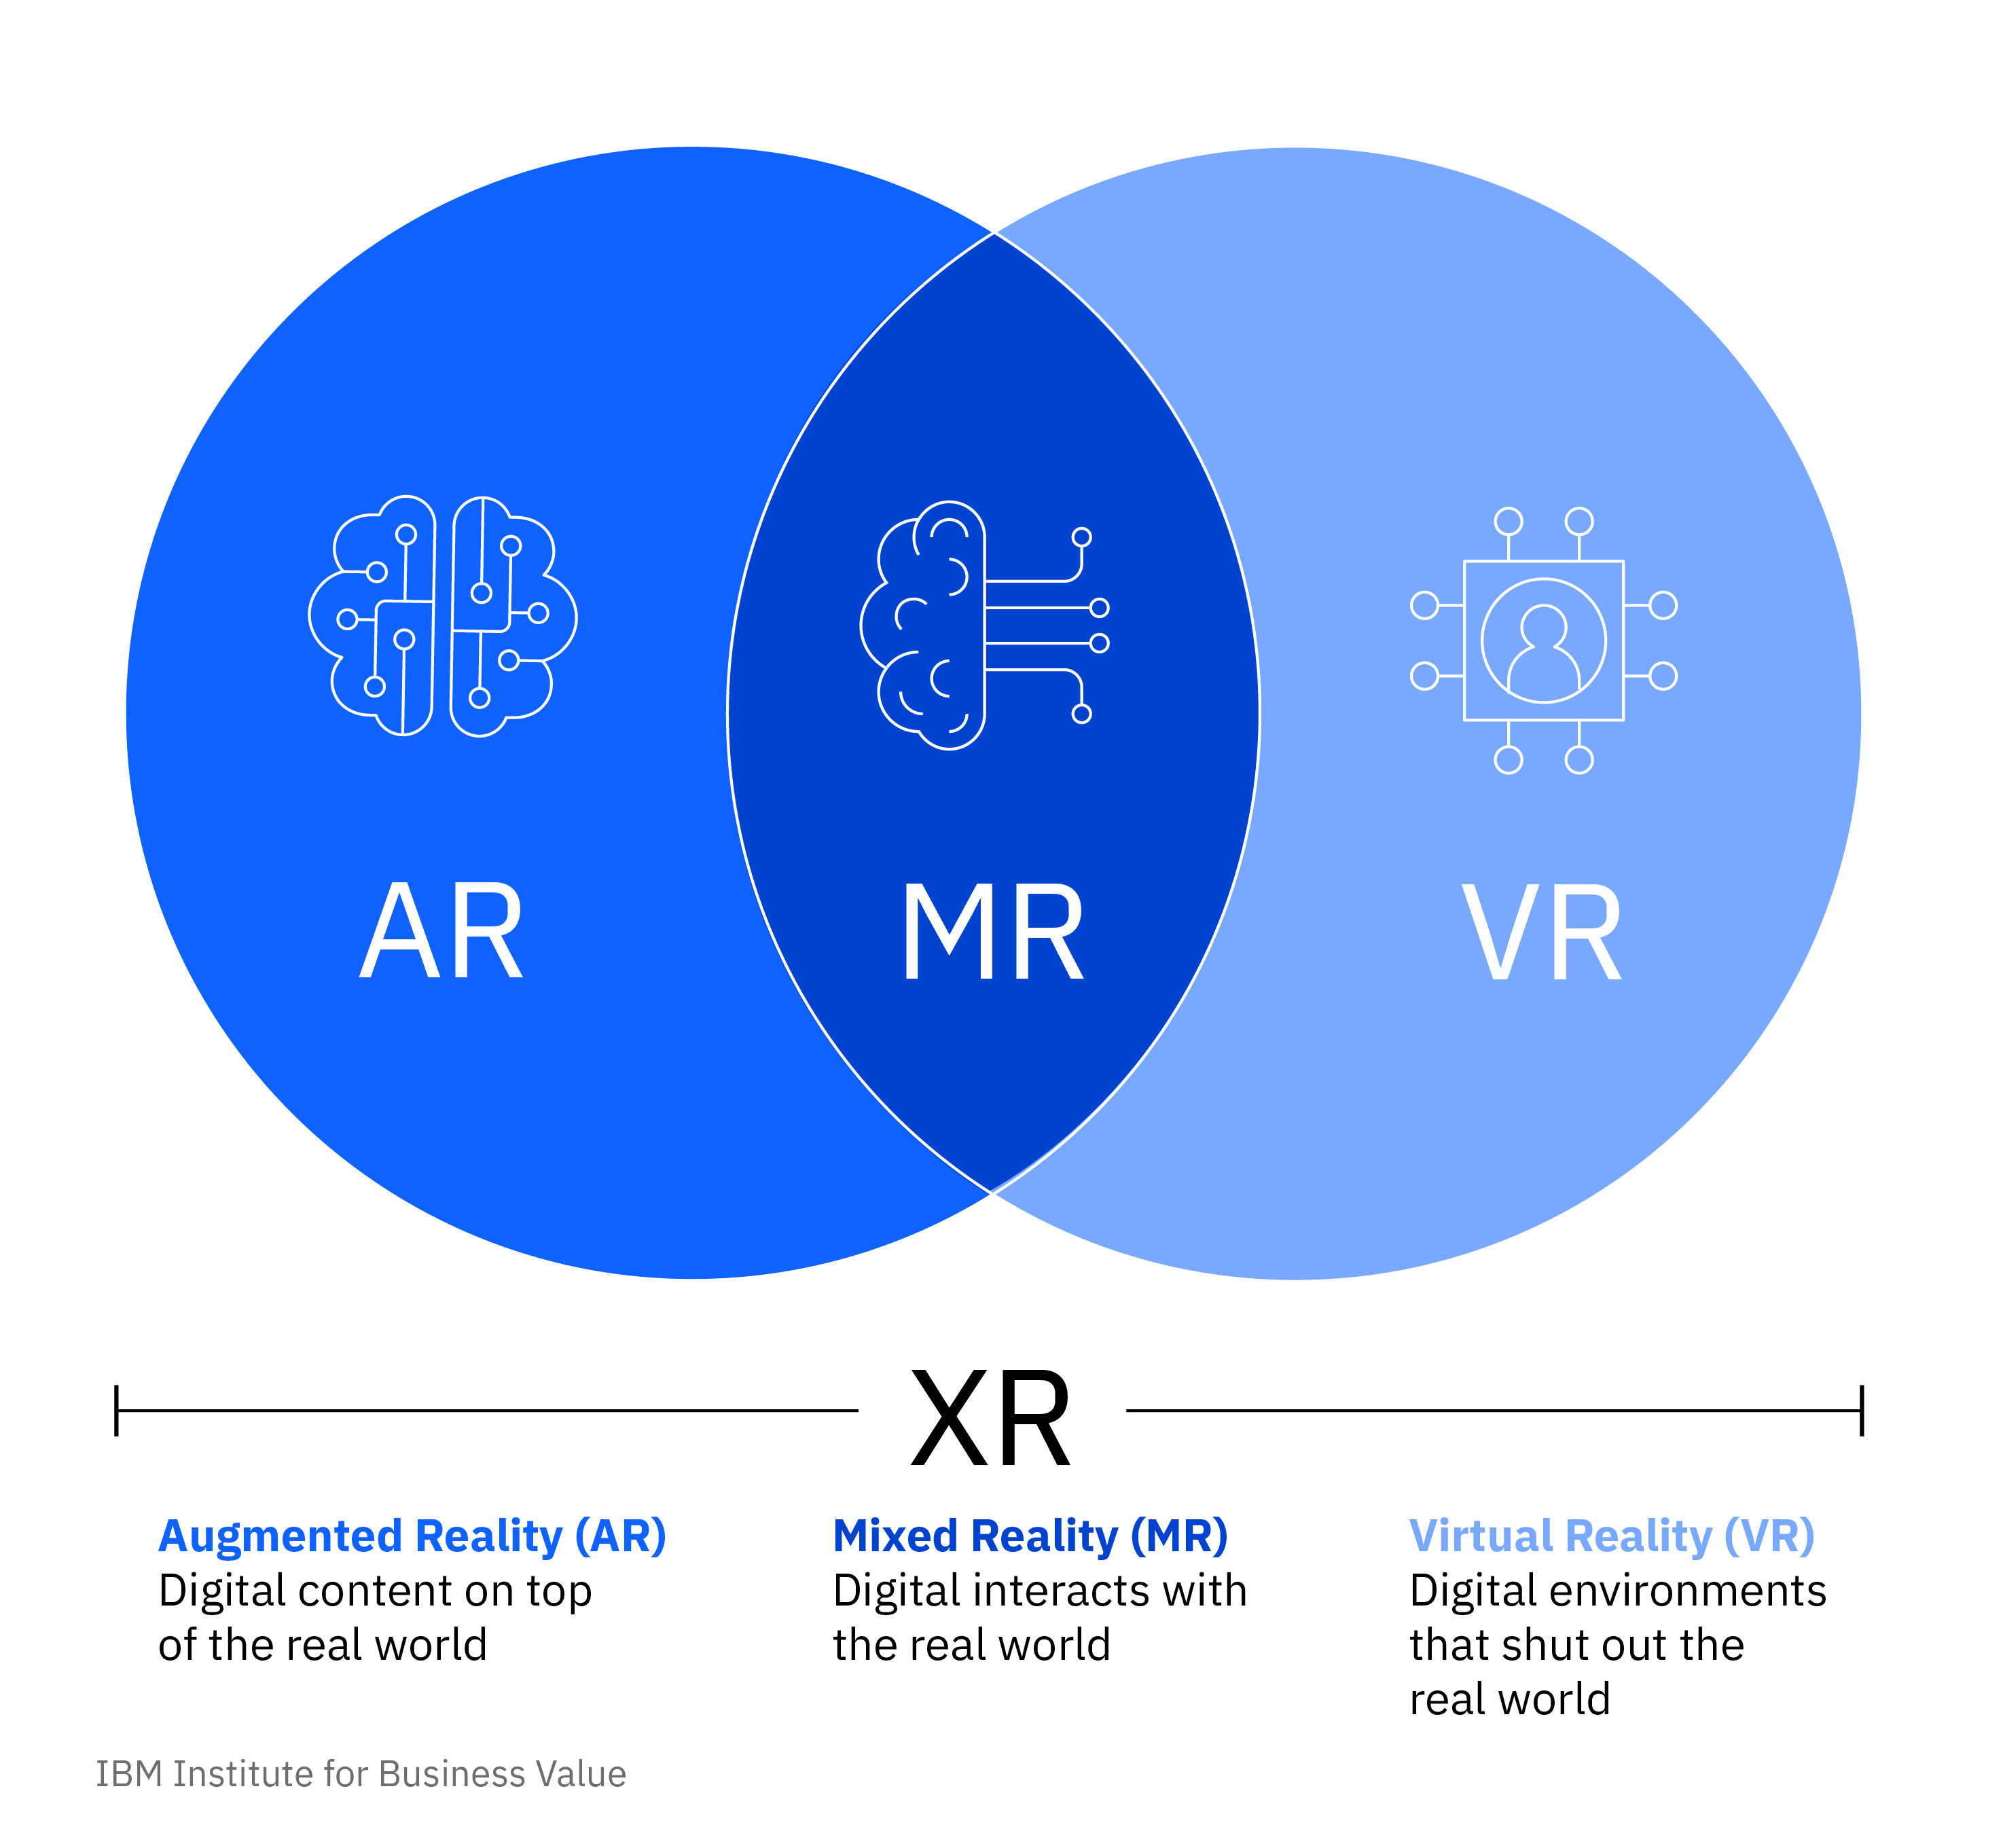
\includegraphics[width=9cm]{ibm_ar.png}}
\caption{Zusammenhang von \gls{xr} zu \gls{vr} und \gls{ar}.\cite{a9}}
\label{xrvrar_fig}
\end{figure}

\subsection{Extended Reality (\gls{xr})}
\gls{xr} (oder auch Cross Reality) ist eine Sammelbezeichnung für alle Kombinationen aus realen und virtuellen Umgebungen,
welche mittels Technologien erzeugt und über Mensch-Maschine-Interaktion gesteuert werden.
Dies schließt auch alle zukünftigen Technologien ein.
Mittels dieser Technologien und zugehörigen Computerprogrammen werden virtuelle, mehrdimensionale Umgebungen erzeugt (\gls{vr}) oder virtuelle Komponenten
der realen Umgebung ergänzt (\gls{ar}) (s. Abbildung \ref{xrvrar_fig}).
Die visuelle Wahrnehmung lässt Umgebungen real erfahren und spricht vermehrt sensorische Reize an.
Werden \gls{xr} als Basis für \gls{sg} verwendet, können diese Reize angesprochen und somit langfristig Informationen und detaillierteres Wissen vermittelt und
vom Gehirn gespeichert werden. Dies verbessert die Qualität des \gls{sg}, bedarf aber eines höheren Aufwands in Vorbereitung und Umsetzung als 2D oder nicht digitale Spiele.

\subsection{Lehrveranstaltung Computergrafik (\gls{cg})}
Im Allgemeinen beschreibt die Lehrveranstaltung \gls{cg} die Modellierung und Erzeugung virtueller Welten, sowie deren Abbildung bzw. Projektion auf 2D-Bilder. Es wird der Informatik zugeordnet.
Die Modellierung und Kombination von komplexen Geometrien und Formen und auch die Berechnung dieser Komponenten sind Teil der \gls{cg}.
Grafische Grundfunktionen, wie Farbdarstellungen oder simple Geometrien, sind Basis dieser Modellierungen.
Beschrieben werden alle diese Modellierungen durch diverse mathematische und computergestützte Algorithmen.
Zudem beinhaltet es die Darstellung von Objekten und Umgebungen in der Ebene, sowie die Abbildung von 3D Umgebungen auf 2D Medien.
Die Computergrafik ist Basis aller \gls{xr} Technologien.
Unabhängig davon, ob einzelne virtuelle Objekte dargestellt werden sollen oder vollständige Umgebungen erzeugt werden, müssen alle Bestandteile
mittels \gls{cg} berechnet und modelliert werden.

Nachfolgend wird ein Beispiel analysiert, welche die hochschuldidaktische Lehre der \gls{cg} mittels \gls{sg} und \gls{xr} unterstützen und fördern kann.

%-----------------------------------------------------------------------------------------------------------------------------------------------
%METHODIKEN

\section{Auswahl an verfügbaren Methoden der \gls{sg}-gestützten Lehre}

Die Variationen an Möglichkeiten der \gls{xr}-gestützten hochschuldidaktischen Lehre ist enorm und wächst stetig an\cite{eduxrvrar2020usa}.
Die Auswahl der verfügbaren und angewendeten Methodiken ist derzeit noch begrenzt.
2D \gls{sg} wird bereits als Lehrmedium verwendet, \gls{xr}-gestützte Medien sind seltener vertreten; 
beide Medien werden zukünftig mehr Einfluss auf die Lehre haben.
Das Besondere an der Integration von \gls{xr} in der Lehre ist die Tatsache,
dass die Lehre der \gls{cg} die Erstellung von \gls{xr} und computergestützten Bildern beschreibt.
Das bedeutet, es kann mithilfe des Mediums selbst den Studierenden vermittelt werden, wie \gls{xr} erstellt und angewendet wird.
Die Bilder und Szenen, die das \gls{sg} den Studierenden mittels \gls{xr} zeigt, sollen beschreiben, wie \gls{xr} funktioniert.
Es bildet somit einen Kreislauf aus der Verwendung von \gls{cg} Inhalten und der Erklärung wie diese Inhalte erstellt werden können.
Anders als in anderen Themenbereichen, wo die Verwendung der \gls{xr} Technologien nur Mittel zum Zweck ist, kann das Mittel hierbei auch die Lehre mitgestalten.

\subsection{2D \gls{sg} Lösung in der hochschuldidaktischen Lehre am Beispiel der Business Simulation \gls{sg}}

Eine Variante der \gls{sg} sind Business Simulation Anwendungen.
Diese sind oft als Planspiel ausgeführt und bieten sich insbesondere in den Lehrveranstaltungen der Wirtschaftswissenschaften an.
Allgemein sind diese i. d. R. als Browser-basierte Varianten ausgeführt und die Benutzerinteraktion beschränkt sich dabei meistens auf das Ausfüllen von Textfeldern und das Lesen von Texten\cite{a11}.
Der \gls{sg} Aspekt entsteht dabei durch das Spielen im Team und gegen gegnerische Teams.
Die Hochschule Osnabrück setzt in der Wirtschaftslehre \gls{sg} bereits erfolgreich ein\cite{a3}.
Studierende werden einzeln oder in Gruppen mit Inhalten konfrontiert, müssen Vorträge halten, für imaginäre Unternehmen Berichte und Protokolle verfassen und ihren
Lernfortschritt festhalten und individuell verbessern\cite{a3}.
Das \gls{sg} kann auch über Kontinente hinweg in verschiedenen Sprachen stattfinden. Somit entsteht nicht nur eine Interaktion mit anderen Studierenden aus der Lehrveranstaltung,
sondern die einzelnen Teilnehmer, das Erlernen von Fachbegriffen und der Umgang mit unternehmensbezogenen Situationen und Aufgaben stehen dabei im Vordergrund\cite{a3}.
Die Spiele werden dabei von der Hochschule erworben, dazu gehören insbesondere die Anbieter TOPSIM, SIMCON GmbH und McGraw-Hill Education, Inc\cite{a3}.
Die Fachhochschule Aachen verwendet ebenfalls TOPSIM im Bereich der Wirtschaftslehre für Informatiker und Ingenieure.
Der Anbieter TOPSIM bietet Cloud-basierte Browser-Anwendungen, bei welchen sich der Nutzer anmeldet, um am 2D Spiel teilzunehmen.
Auch gedruckte Ausgaben sind möglich. Eine \gls{xr} Integration oder Umsetzung ist bisher nicht vorgesehen.
Die Lehrenden der Hochschule Osnabrück konnten eine Verbesserung unter den Studierenden feststellen, die ohne \gls{sg} weniger hervorragende Leistungen erbringen.
Leistungsstärkere Studierende profitieren weniger, jedoch wird bei allen Studierenden eine erhöhte Sozialkompetenz festgestellt.
Nachteilig sind die hohen Kosten für die Spiellizenzen, die komplexe Einarbeitung in das System und die oft unübersichtliche Aufgabengestaltung,
die Studierende zur Prokrastination verleitet\cite{a3}.
Derartige Spiele z.B. Wirtschaftssimulationen\cite{a11} gilt es nun in \gls{xr} zu transferieren und die Lehre der Wirtschaftswissenschaften durch \gls{cg} zu erweitern, ohne die Vorteile des Spiels zu verlieren.

\subsection{Aspekte des \gls{sg}s in der \gls{cg} Lehre und eine mögliche Umsetzungsstrategie mittels \gls{xr}}

Bevor ein \gls{sg} für eine Lehrveranstaltung erstellt werden kann, müssen nach\cite{a14} drei Teilbereiche umgesetzt werden:
Realität (wie das Spiel mit der physischen Welt verbunden ist), Bedeutung (welcher Wert erreicht werden soll)
und Spiel (wie man spielerische Aktivitäten schafft)\cite{a14}.
Feng, Amor, Gonzales und Lovreglio\cite{a15} formulieren elf Fragen, um diese drei Hauptaspekte zu erlangen.
Insbesondere pädagogische und verhaltensbezogene Aspekte und Ergebnisse stehen dabei im Vordergrund.

\begin{table}[]
\caption{Systematische literaturbezogene Forschungsfragen nach\cite{a14}}
\begin{tabular}{|l|l|}
\hline
1  & Welche Unterrichtsmethoden werden verwendet?                                                                                                                           \\ \hline
2  & Welche Lernziele werden verfolgt?                                                                                                                                      \\ \hline
3  & Wie sehen die Lernmaßnahmen aus?                                                                                                                                       \\ \hline
4  & Welche Ergebnisse bezüglich des Verhaltens werden erzielt?                                                                                                                                \\ \hline
5  & Wie sehen die Verhaltensmaßnahmen aus?                                                                                                                                      \\ \hline
6  & Welche Navigations-Lösungen gibt es?                                                                                                                                   \\ \hline
7  & Wie werden Sinne angeregt?                                                                                                                                             \\ \hline
8  & \begin{tabular}[c]{@{}l@{}}Welche narrativen Methoden gibt es, um Teilnehmer zu\\ermutigen, der Spielhandlung zu folgen und sie abzuschließen?\end{tabular} \\ \hline
9  & Wie werden Gefahren simuliert?                                                                                                                                         \\ \hline
10 & \begin{tabular}[c]{@{}l@{}}Gibt es nicht spielbare Charaktere und was tragen\\sie zum Spiel bei?\end{tabular}                                                                                              \\ \hline
11 & Wie kann man die Erfahrungen der Teilnahme bewerten?                                                                                                                   \\ \hline
\end{tabular}
\label{table:firsttable}
\end{table}
%\cite{a14}

Die Varianz der Darstellung der Lehre der \gls{cg} ist groß. 
Eine mögliche Umsetzung wäre die Modellierung und Berechnung eines eigenen \gls{xr} Erlebnisses,
welches mit neu erlernten Funktionen immer komplexer wird. Angefangen beim schwarzen oder durchsichtigen Bildschirm lassen sich Aufgaben und Fragen stellen,
die den Studierenden neue mathematische Funktionen vermitteln und aus diesen Objekte, Strukturen und Segmente erzeugen. 
Studierende können ihre Berechnung bzw. das modellierte Ergebnis direkt auf der \gls{vr} sehen und vergleichen und bekommen unmittelbar Feedback. 
\gls{cg} wird mittels \gls{xr} für Studierende greifbar gemacht. 
Die Komplexität wird langsam gesteigert, Funktionen und Modellierungen überlagern sich und ergeben ein Gesamtwerk, welches das Ziel der Vorlesung ist. 

Bezieht man die Forschungsfragen aus Tabelle \ref{table:firsttable} auf die Lehre der \gls{cg} und die Software des \gls{xr} auf die Erstellung eines solchen Erlebnisses,
lässt sich u.a. diese Umsetzungsmöglichkeit finden, welche im nachfolgenden Absatz detaillierter aufgegriffen wird:

\begin{itemize}
\item Die Lehre beinhaltet Methoden und Schwierigkeiten der Abbildung einer dreidimensionalen Szene (real oder modelliert) auf ein zweidimensionales Ausgabegerät (Bildschirm)\cite{scholl}.
\item 1: Mittels \gls{xr} soll \gls{cg} erklärt werden; da \gls{xr} ein Teilgebiet der \gls{cg} ist, kann hier eine aufbauende Methodik verwendet werden,
beispielsweise angefangen vom einfachen Farbton und dessen Berechnungen über Geometrien und Modellierungen bis hin zu Konvertierungen.
Programme und Funktionen, welche Studierende selbst programmieren, können direkten Einfluss auf das \gls{xr} Ergebnis haben.
\item 2: Neben graphischen Grundfunktionen werden 3D Objekte geometrisch modelliert und diese auf 2D Ausgabegeräten dargestellt und die GPU-Programmierung eingeführt.
\item 3: Studierende erkennen Zusammenhänge zwischen mathematischen Funktionen und deren Parametern zur Darstellung von Objekten.
\item 4: Ziel ist das Verständnis der mathematischen Verfahren und der Algorithmen, die zur Erzeugung von Grafiken in der Computergrafik eingesetzt werden;
Computergrafiken sollen unter Anwendung der erlernten Verfahren programmiert werden.
\item 5: Studierende erarbeiten einzeln und in Gruppen schrittweise einzelne Funktionen und erzielen zum Schluss ein \gls{xr} Gesamtergebnis.
\item 6: Neben der Strukturierung durch vorgegebene mathematische Funktionen, sortiert nach Komplexität,
erfolgt die Hardware-Steuerung mittels händischer Steuerung mit aktiver Sensorik.
\item 7: Sinne werden durch die \gls{cg} vorrangig grafisch angesprochen.
Akustisch können Aktionen, Anwendungen von Gleichungen und Funktionen untermalt werden und abhängig vom Ton positive und negative Ergebnisse betont werden.
Haptisch und olfaktorisch entfallen bei der hier gewählten Lösung.
\item 8: Das Ziel des Spiels ist ein Gesamtwerk; eine Transformation der eigenen Funktionen und 3D Modellierungen auf eine 2D Oberfläche;
Spieler werden angehalten, ihre Oberfläche themenabhängig mit sämtlichen verfügbaren Funktionen kreativ zu gestalten.
\item 9: Gefahren, Schwierigkeiten und Fehler werden durch grafische Fehldarstellungen oder fehlerhafte Programmierung betont
und akustisch untermalt.
\item 10: Lehrende und Mentoren, können von außen das Spiel beeinflussen und unterstützend zur Seite stehen.
\item 11: Bewertet werden das Gesamtergebnis und die Integration aller verfügbaren Komponenten und deren Kombination.
Studierende sollen ihr Ergebnis parametrisierbar und veränderlich gestalten und somit beweisen, dass sie die Varianz der \gls{cg} verstanden haben.
\end{itemize}

Die aufgeführten Stichpunkte beinhalten eine Lösungsmöglichkeit der Umsetzung der Lehre der \gls{cg} mittels \gls{xr}.
Weitere Möglichkeiten, wie Rollenspiele oder Abenteuer mit mathematischen und modellierbaren Hindernissen und Aufgaben, sind ebenso möglich.
Nachfolgend wird die Umsetzung eines eigenen \gls{cg} Projektes mit \gls{xr} als Anzeigemedium mittels einer verfügbaren Software betrachtet.


%-----------------------------------------------------------------------------------------------------------------------------------------------
%SHADER

\subsection{Umsetzung mittels einer beispielhaften kommerziell-verfügbaren Software-Applikation}

Am Beispiel der Shader-Erstellung wird nun die zuvor definierte Umsetzung des \gls{sg}s erläutert. 
Ein wichtiger Bestandteil der \gls{cg} ist die Entwicklung von Shadern. 
Dies sind kleine Programme, welche direkt auf dem Grafikbeschleuniger eines Computers ausgeführt werden können.
Die Darstellung (Rendering) von 3D Objekten auf dem Anzeigegerät wird maßgeblich durch Shader beeinflusst. 
Hierbei durchläuft ein Objekt eine Reihe von mathematischen Operationen, welche die visuelle Darstellung beeinflussen (Renderpipeline). 
So lassen sich unter anderem Licht-Reflexionen auf das Objekt projizieren oder Weichzeichner-Effekte darstellen.
Das Entwickeln solcher Programme ist ein wichtiger Bestandteil der \gls{cg} Lehrveranstaltung.
Hier erstellen die Studierenden im Verlauf eines Projekts verschiedene Shader-Programme.
Im Rahmen der Vorlesung wird der Aufbau dieser anhand von Beispielen exemplarisch gezeigt und die Studierenden können diese Beispiele im Nachhinein nachvollziehen.

Es bieten eine visuelle Repräsentation der erstellten Renderpipeline und deren Einzelschritte diverse Vorteile.
Änderungen eines Schrittes können direkt visuell nachvollzogen werden, welche allein durch den Quellcode nicht direkt ersichtlich sind.
Diese Darstellungsform unterstütz einen effizienten Wissenstransfer, da das Verständnis einzelner Funktionen sowie deren Zusammenspiel interaktiv dargestellt wird.
Exemplarisch bietet die Shadertool-Software\cite{shadertool} solch eine Darstellung an.
Hier wird die Renderpipeline in einem 2D-Modus visuell dargestellt (s. Abbildung \ref{shadertool1_fig}) und Änderungen werden fortlaufend visualisiert.

\begin{figure}[htbp]
\centerline{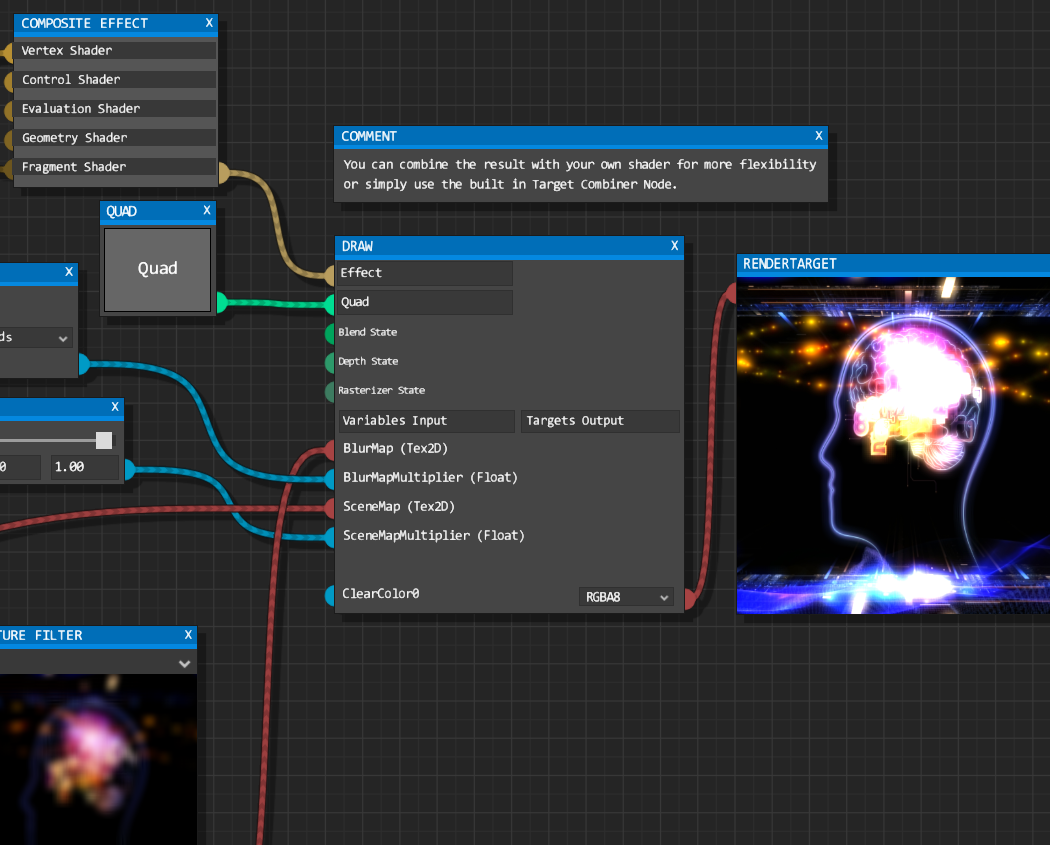
\includegraphics[width=8cm]{shadertool_1.png}}
\caption{Shadertool Software im 2D Modus\cite{shadertool}}
\label{shadertool1_fig}
\end{figure}

Da im Bereich der \gls{cg} und somit auch in der \gls{cg} Lehrveranstaltung nahezu ausschließlich mit 3D Objekten gearbeitet wird,
bietet sich zusätzlich die Verwendung der \gls{xr} Technologie an.
Mit dieser ist es möglich, die erstellten Objekte, Grafiken und Shader-Effekte immersiv zu erleben und zudem qualitativ beurteilen zu können.

Am Beispiel der Shadertool Software\cite{shadertool} ist es möglich, diese in einen \gls{vr}-Modus zu schalten, welcher zum einen die erstellte Renderpipeline räumlich darstellt
und zum anderen die visuellen Darstellungen der Objekte erlebbar macht.
Somit ist es schnell möglich, visuelle Unstimmigkeiten, welche durch die Shader-Programme erzeugt werden, zu identifizieren, jedoch bietet dieser Ansatz keine direkten \gls{sg} Möglichkeiten.
Die Software wurde als simples Werkzeug konzipiert.
Um solch eine Software mittels \gls{sg} Ansatz verwenden zu können, müssen spielerische Elemente sowie gezielte Aufgabenstellungen für zu erreichenden Lernziele hinzugefügt werden.

\subsection{Analyse der Umsetzung}

Bei dem eben erläuterten Shader-Tool handelt es sich um eine spezialisierte Lösung, welche nur für diesen Einsatzbereich
verwendet werden kann. Jedoch ist der Aufwand zur Umsetzung bis in die aktive Lehrveranstaltung arbeitsintensiv.
Zudem gibt es im Bereich der Shader-Programme, insbesondere in der \gls{cg}, kaum Möglichkeiten, diese auch in anderen Veranstaltungen einzusetzen.
Jedoch bieten diese Lösungen den Vorteil, dass diese auf den bestmöglichen Lernerfolg ausgelegt werden können.
Bei der Verwendung solcher Software mit zusätzlicher \gls{xr} Komponente (auch ohne das Ziel eines expliziten \gls{sg} Ansatzes), ist es möglich, mit wenig Aufwand eine immersive Erfahrung zu erzeugen.
Dies ist insbesondere auf das Themengebiet der \gls{cg} zurückzuführen, in der die Lehrinhalte und insbesondere das Erstellen und Visualisieren von 3D-Objekten, schnell grafisch dargestellt werden können.
Viele der verfügbaren 3D-Grafikprogramme (z. B. Blender\cite{blender} ab Version 3.0) und 3D-Engines (z. B. Unity\cite{unity3d}) unterstützen bereits \gls{xr} Funktionen sowohl in der Darstellung von 3D-Szenen und Objekten als auch während der Bearbeitung.
Da einige dieser Software-Lösungen bereits in der \gls{cg} eingesetzt werden, ist hier eine Integration von \gls{xr} ohne viel Aufwand möglich.


Ein zusätzlicher Nachteil dieser Software und der oben genannten Alternativen ist, dass diese leistungsstarke Hardware erfordern.
Hier wird ein für die Anwendung geeigneter Computer, welcher mit einem leistungsstarken Grafikbeschleuniger ausgestattet ist, benötigt.
Zudem muss auch ein \gls{vr}-Headset verwendet werden, welches den Anforderungen der Software gerecht wird.
Diese Hardwarelimitierungen erschweren die Skalierbarkeit in Lehrveranstaltungen mit mehreren Studierenden und Gruppenarbeiten.

Um dieses Problem zu lösen, muss auf kostengünstige Hardware zurückgegriffen werden, um eine kostengünstige Skalierung zu ermöglichen.
Die Verwendung eines modernen Mobiltelefons (smartes Endgerät), welche über hochauflösende Bildschirme, sowie schnelle Prozessoren verfügen, können hier Abhilfe schaffen.
Zusätzlich wird eine Halterung benötigt, welche im Zusammenspiel mit dem Mobiltelefon als \gls{vr}-Headset fungiert.
Ein bekanntes Beispiel für eine kostengünstige Lösung, ist das von Google entwickelte Open-Source Projekt Google Cardboard\cite{googlecardboard}.

Hier wird das Mobiltelefon in einen einfachen Papierrahmen eingehängt, welcher dann vor den Augen befestigt werden kann.
Somit steht eine einfache Möglichkeit \gls{vr}-Inhalte mittels spezieller dafür angepasster Applikationen darstellen zu können zur Verfügung.

Durch den einfachen Aufbau des Headsets bietet dies keine weiteren Interaktionsmöglichkeiten für die Nutzer.
Hier kann nur sehr eingeschränkt direkt mit dem Inhalt interagiert werden, welches einen Einsatz bei Spielen oder \gls{cg}-Anwendungen erschwert.


Dazu können verschiedene externe Eingabegeräte verwendet werden.
U.a. ist es möglich mittels Hand-Controller, Handgesten an die Anwendung zu übermitteln.
Alle externen Controller werden dabei i. d. R. kabellos per Bluetooth mit dem Mobiltelefon gekoppelt.
Somit ist auch ein Ausleihen solcher Controller an die Studierenden möglich.

Da bei dieser Lösung ein Mobiltelefon zum Einsatz kommt, kann die in diesem Beispiel untersuchte Shader-Tool Software\cite{shadertool} nicht auf dieser Hardware-Plattform ausgeführt werden.
Es gibt keine direkte Alternative, jedoch zeigen Webseiten, wie z. B. Shadertoy\cite{shadertoy}, dass es möglich ist, eindrucksvolle Shader performant im Browser darzustellen.
Dabei können verschiedene Shader direkt im Browser erstellt und bearbeitet werden und können somit auch direkt auf einem Mobiltelefon angezeigt werden.
Lediglich die \gls{xr} oder insbesondere \gls{vr} Unterstützung fehlen.

Andere Software-Pakete, wie Unity\cite{unity3d}, bieten hier bereits eine vollständige Entwicklungsumgebung für \gls{xr} Anwendungen an.
Diese können nach dem Erstellen einer Applikation auf das Mobiltelefon geladen werden und z. B. mittels des Google Cardboard-Headsets\cite{googlecardboard} ausprobiert werden.

Eine solche Lösung eignet sich für eine weitere Untersuchung im Einsatz in der \gls{cg}-Lehre.
Da es sich zum einen um eine kostengünstige, gut skalierbare \gls{vr}-Plattform handelt und es zum anderen bereits einige Softwarekomponenten gibt, 
welche sich mit den Lehrinhalten der \gls{cg} verwenden lassen und mit dieser kompatibel sind.
Die Skalierbarkeit des Systems macht es nicht nur für neue Lerninhalte einfacher erweiterbar, sondern auch für weitere, zukünftige \gls{xr} Technologien modular integrierbar.




%-----------------------------------------------------------------------------------------------------------------------------------------------
%VERGLEICHE

\section{Evaluation}

Ein wichtiger Punkt bei der Verwendung von \gls{sg} in der Lehre, ist die anschließende Evaluation des Lernerfolgs.
Zusätzlich zur Wissensvermittlung ist auch die Akzeptanz des Zielpublikums eine wichtige Messgröße.
Hierzu hat die Hochschule Osnabrück eine Handlungsempfehlung aus gewonnenen Erkenntnissen aus dem \gls{gbl} Gebiet zusammengestellt\cite{a3}.
Diese umfasst zudem die folgenden Punkte, um \gls{sg} in der Lehre evaluieren zu können.
Das Einholen von Feedback von den Lehrenden sowie von den Studierenden ist essenziell.
Dies geschieht zum einen mit Teilnehmern, bei denen eine Wissensvermittlung mittels \gls{sg} erfolgte und zum anderen mit einer zweiten Gruppe,
bei der die Wissensvermittlung durch klassische Aufgaben umgesetzt wurde.

Dieser Feedback-Prozess ist insbesondere bei der Wissensvermittlung durch \gls{xr} Technologien relevant.
Jeder Studierende nimmt die \gls{xr} Umgebung unter Umständen anders wahr und interagiert unterschiedlich mit dieser.
Anders als bei einer fest vorgegebenen \gls{sg} Anwendung, welche unter Umständen nur wenige Interaktionsmöglichkeiten bietet, ist die \gls{xr} Technologie
darauf ausgelegt, den Teilnehmern mehr Interaktionsmöglichkeiten zu bieten.

Demnach muss auch der Feedback-Prozess angepasst werden. Hierzu kann nicht nur auf ein reines Feedback der Teilnehmer,
sondern es muss auch auf eine externe Gruppe zugrückgegriffen werden, welche die Teilnehmerinteraktionen während der Anwendung in \gls{xr} beobachtet.
Diese Erkenntnisse, wie die Teilnehmer in der \gls{xr} Umgebung interagieren, geben zusätzlich zu dem oben genannten Feedback-Prozess Aufschluss,
ob die Anwendung den Teilnehmerfokus auf die Wissensvermittlung lenkt.

Für die Evaluation im Bereich der Lehre der \gls{cg} empfiehlt sich eine Evaluation des Gesamtergebnisses.
Diese beinhaltet die von den Studierenden erstellte \gls{xr} Umgebung und die darin verwendeten \gls{cg} Komponenten und Funktionen.
Um Studierende von der Verwendung der \gls{xr} Technologie in der Lehre nicht auszuschließen, ist eine zusätzliche Gruppe von Betreuern, wie Tutoren, nötig,
welche den Prozess und die Beteiligung der Studierenden begleiten.

Zudem sollte keine Momentaufnahme als Evaluation betrachtet werden, sondern ein Vergleich der Ergebnisse der Teilnehmergruppen über verschiedene Semester zu Rate gezogen werden,
um Aufschluss über mögliche Änderungen, Verbesserungen oder gar Verschlechterungen geben zu können.

Abschließend ist festzuhalten, dass u. U. nicht jeder Studierende an dem \gls{xr} Erlebnis teilnehmen möchte oder dieses nicht anwenden kann. 
Zudem dürfen jene, welche das Projekt im Verlauf des Semesters nicht abschließen können, nicht ausgeschlossen werden.
Für diese muss ein konservativer Lösungsweg angeboten werden.
%-----------------------------------------------------------------------------------------------------------------------------------------------
%FAZIT

\section{Fazit und Ausblick}


\gls{sg}, insbesondere in Verbindung mit \gls{xr}, bietet in der hochschuldidaktischen Lehre ein großes Potential.
Die z. T. bereits etablierte Anwendung des 2D \gls{sg}s in der Wirtschaftslehre hat bewiesen, 
dass die Methodik sowohl umsetzbar ist, als auch Studierende aller Leistungsbereiche fördert. 
Anhand der exemplarischen Umsetzungsmöglichkeit in der \gls{cg} Lehrveranstaltung wurde gezeigt,
dass es möglich ist, \gls{xr} Technologien so einzusetzen, dass diese eine Wissensvermittlung unterstützen. 
Die Varianz an Umsetzungsmöglichkeit ist enorm; 
da \gls{xr} ein Teilbereich der \gls{cg} ist, bietet sich hier ein direkter Zusammenhang zwischen beiden Mitteln an.
Die Lehre der \gls{cg} kann mittels \gls{xr} erklärt werden.
Die Studierenden erstellen eine \gls{xr} Umgebung und erlernen zeitgleich Methodiken der \gls{cg}. 
Somit entsteht ein effizienter Kreislauf. 
Eine mögliche Umsetzungsform ist hierbei die Verwendung von bereits bestehender Software, welche keinerlei spielerische Elemente besitzt.
Diese kann durch eine Anpassung und Weiterentwicklung mit derartigen Elementen versehen werden um somit den Anforderungen der \gls{cg} gerecht zu werden.
Die im Beispiel analysierte Software, bietet zudem direkt eine Unterstützung für den \gls{xr} Modus und eignet sich somit für eine Evaluation.

Andere Software-Applikationen, welche sich für die Verwendung in der \gls{cg} Lehrveranstaltung eignen, bringen diese Features i. d. R. nicht mit.
Einige andere können die zuvor erstellten Modelle bzw. 3D-Welten in einer \gls{xr} Umgebung darstellen.
Das Erstellen dieser geschieht im 2D-Modus an einem PC.
Hier bietet diese Symbiose zwischen der Erstellung und dem Betrachten im \gls{xr} den Vorteil, dass die erlernten Konzepte immersiv erforscht werden können.
Dabei können die positiven Erfahrungen aus den bereits angewendeten 2D-\gls{sg}s übernommen und durch die Erweiterung mittels \gls{xr} gesteigert werden.

Nachteilig ist hierbei, dass all diese Ansätze mit einem hohen Arbeits- und Kostenaufwand verbunden sind.
Potenzielle Software, welche nicht über \gls{sg} Elemente sowie \gls{xr} Funktionalitäten verfügt, muss aufwändig angepasst werden.

Ebenso stellt die benötigte \gls{xr}-Hardware einen Kostenfaktor dar, da bestimmte Spezifikationen erfüllt werden müssen.


Eine Möglichkeit ist die Verwendung kostengünstiger \gls{xr} Ansätze, welche ein modernes Mobiltelefon als Grundlage verwenden.
Diese sind heutzutage in der Lage, komplexe \gls{xr}-Anwendungen auszuführen, bieten aber ohne externe Eingabegeräte kaum Möglichkeiten einer Interaktion mit der \gls{xr} Umgebung.
Durch die Ergänzung von z. B. Hand-Controllern, welche an Studierende verliehen werden können, ist es möglich in der \gls{cg} Lehrveranstaltung ein nahezu vollständiges \gls{xr} Erlebnis zu bieten.


Abschließend ist festzuhalten, dass eine Integration von \gls{sg} Ansätzen in die Lehre und insbesondere die Integration von \gls{xr} in die Lehre der \gls{cg} sinnvoll und zukunftsorientiert ist
und zudem Wissen effizienter vermittelt.
Studierende und Lehrende profitieren. Hürden, wie Hardware und Arbeitsaufwand, erschweren diese, sind aber nach einmaliger Umsetzung dauerhaft anwendbar.
Eine Integration ist somit zu empfehlen.



%-----------------------------------------------------------------------------------------------------------------------------------------------
\begingroup

%\setstretch{1.05}
\begin{thebibliography}{00}
\bibitem{eduxrvrar2020usa} Thomas Alsop: "Leading applications of immersive technologies in the education sector in the next two years according to XR/AR/VR/MR industry
experts in the United States in 2020", in: Internetseite Statista, URL: https://www.statista.com/statistics/1185078/applications-immersive-technologies-xr-ar-vr-mr-education/, Abruf am 17.11.2021.

\vskip 0.05in
\bibitem{evallearningmixedreality2020} Y. M. Tang; K. M. Au; H. C. W. Lau; G. T. S. Ho, C. H. Wu; "Evaluating the effectiveness of learning design with mixed reality (MR) in higher education", Springer-Verlag London Ltd, 28.02.2020

\vskip 0.05in
\bibitem{a7} Linda Stege, Giel van Lankveld, Pieter Spronck; "Serious Games in Education", International Journal of Computer Science in Sport, 2011

\vskip 0.05in
\bibitem{fabulagames} Fabula Games, "LERNEN KANN SOOO BUNT SEIN", in: Internetseite Fabula Games, URL: https://fabula-games.de/, Abruf am 22.11.2021.

\vskip 0.05in
\bibitem{a3} Axel Jacob, Frank Teuteberg; "Game-Based Learning, Serious Games, Business Games und Gamification –Lernförderliche Anwendungsszenarien, gewonnene Erkenntnisse und Handlungsempfehlungen", Springer Fachmedien Wiesbaden GmbH, 2017

\vskip 0.05in
\bibitem{grundlagencg2001} Thomas Strothotte, Stefan Schlechtweg; "Grundlagen der Computergraphik", 2001

\vskip 0.05in
\bibitem{shadertool} Stefan Kraus, Timo Armbruster; "ShaderTool", in: Internetseite Steam, URL: https://store.steampowered.com/app/314720/ShaderTool/, Abruf 02.12.2021

\vskip 0.05in
\bibitem{a9} IBM Institute for Business Value; "Extended Reality (XR) can boost workforce efficiency and resilience by reimagining how work is done.", in: Internetseite IBM Institute for Business Value, URL: https://www.ibm.com/thought-leadership/institute-business-value/report/ar-vr-workplace, Abruf am 22.11.2021.

\vskip 0.05in
\bibitem{a10} Joseph F. Frederick; "Defining Serious Games", in: Internetseite flowleadership, URL: https://flowleadership.org/serious-games/, Abruf am 22.11.2021.

\vskip 0.05in
\bibitem{blender} Blender Foundation; "Blender", in: Internetseite Blender, URL: https://wiki.blender.org/wiki/Reference/Release\_Notes/3.0, Abruf am 22.11.2021.

\vskip 0.05in
\bibitem{unity3d} Unity Technologies; "Unity VR", in: Internetseite Unity Technologies, URL: https://unity.com/de/case-study\#games-vr, Abruf am 22.11.2021.

\vskip 0.05in
\bibitem{a11} TOPSIM; "TOPSIM-General Management-Teilnehmerhandbuch", in: Internetseite TOPSIM, URL: https://www.css.msm.uni-due.de/fileadmin/Dateien/MSM/Topsim-Gr8/01\_General\_Management\_Teilnehmerhandbuch\_STD\_15\_3.pdf, Abruf am 22.11.2021.

\vskip 0.05in
\bibitem{a14} Zehnan Feng, Robert Amor, Vicente Gonzales, Ruggiero Lovreglio; "Immersive Virtual Reality Serious Games for Evacuation Training and Research: A Systematic Literature Review", ResearchGate, 05.2018

\vskip 0.05in
\bibitem{a15} Rüppel, Schatz; "Designing a BIM-based serious game for fire safety evacuation simulations"; Advanced Engineering Informatics; 2011

\vskip 0.05in
\bibitem{googlecardboard} Google LLC; "Google Cardboard", in: Internetseite google.com, URL: https://arvr.google.com/intl/de\_de/cardboard/apps/, Abruf am 22.11.2021.

\vskip 0.05in
\bibitem{shadertoy} Inigo Quilez, Pol Jeremias; "Shadertoy", in: Internetseite shadertoy.com, URL: https://www.shadertoy.com, Abruf am 22.11.2021.

\vskip 0.05in
\bibitem{scholl} Ingrid Scholl, "Computergrafik" in: Internetseite Vorlesung Computergrafik von Fr. Prof. Scholl, Ingrid; URL: https://www.fh-aachen.de/menschen/scholl/lehre/computergrafik, Abruf am 01.12.2021.




\end{thebibliography}
\endgroup

\end{document}


